\documentclass{sigchi}

% Use this command to override the default ACM copyright statement (e.g. for preprints). 
% Consult the conference website for the camera-ready copyright statement.


%% EXAMPLE BEGIN -- HOW TO OVERRIDE THE DEFAULT COPYRIGHT STRIP -- (July 22, 2013 - Paul Baumann)
% \toappear{Permission to make digital or hard copies of all or part of this work for personal or classroom use is 	granted without fee provided that copies are not made or distributed for profit or commercial advantage and that copies bear this notice and the full citation on the first page. Copyrights for components of this work owned by others than ACM must be honored. Abstracting with credit is permitted. To copy otherwise, or republish, to post on servers or to redistribute to lists, requires prior specific permission and/or a fee. Request permissions from permissions@acm.org. \\
% {\emph{CHI'14}}, April 26--May 1, 2014, Toronto, Canada. \\
% Copyright \copyright~2014 ACM ISBN/14/04...\$15.00. \\
% DOI string from ACM form confirmation}
%% EXAMPLE END -- HOW TO OVERRIDE THE DEFAULT COPYRIGHT STRIP -- (July 22, 2013 - Paul Baumann)

\toappear{Permission to make digital or hard copies of all or part of this work for personal or classroom use is  granted without fee provided that copies are not made or distributed for profit or commercial advantage and that copies bear this notice and the full citation on the first page. Copyrights for components of this work owned by others than ACM must be honored. Abstracting with credit is permitted. To copy otherwise, or republish, to post on servers or to redistribute to lists, requires prior specific permission and/or a fee. Request permissions from permissions@acm.org. \\
{\emph{L@S'15}}, March 14-15, 2015, Vancouver, Canada. \\
Copyright \copyright~2015 ACM ISBN/15/03...\$15.00. \\
DOI string from ACM form confirmation}

% Arabic page numbers for submission. 
% Remove this line to eliminate page numbers for the camera ready copy
% \pagenumbering{arabic}


% Load basic packages
\usepackage{balance}  % to better equalize the last page
\usepackage{graphicx} % for EPS, load graphicx instead
\usepackage{times}    % comment if you want LaTeX's default font
\usepackage{url}      % llt: nicely formatted URLs
\usepackage{epstopdf}

% llt: Define a global style for URLs, rather that the default one
\makeatletter
\def\url@leostyle{%
  \@ifundefined{selectfont}{\def\UrlFont{\sf}}{\def\UrlFont{\small\bf\ttfamily}}}
\makeatother
\urlstyle{leo}


% To make various LaTeX processors do the right thing with page size.
\def\pprw{8.5in}
\def\pprh{11in}
\special{papersize=\pprw,\pprh}
\setlength{\paperwidth}{\pprw}
\setlength{\paperheight}{\pprh}
\setlength{\pdfpagewidth}{\pprw}
\setlength{\pdfpageheight}{\pprh}

% Make sure hyperref comes last of your loaded packages, 
% to give it a fighting chance of not being over-written, 
% since its job is to redefine many LaTeX commands.
\usepackage[pdftex]{hyperref}
\hypersetup{
pdftitle={Game Theory based Peer Grading Mechanisms for MOOCs},
pdfauthor={LaTeX},
pdfkeywords={MOOC, game theory, mechanism design, peer grading, learning at scale},
bookmarksnumbered,
pdfstartview={FitH},
colorlinks,
citecolor=black,
filecolor=black,
linkcolor=black,
urlcolor=black,
breaklinks=true,
}

% create a shortcut to typeset table headings
\newcommand\tabhead[1]{\small\textbf{#1}}


% End of preamble. Here it comes the document.
\begin{document}

\title{Game Theory based Peer Grading Mechanisms for MOOCs}

\numberofauthors{2}
\author{
  \alignauthor William Wu\\
    \affaddr{Acton Boxborough Regional High School}\\
    \affaddr{36 Charter Rd\\ Acton, MA 01720, USA}\\
    \email{willy.vvu@gmail.com}
  \alignauthor Nicolaas Kaashoek\\
    \affaddr{Lexington High School}\\
    \affaddr{251 Waltham Street\\ Lexington, MA 02421, USA}\\
    \email{nick.kaashoek@gmail.com}
}

\maketitle

\begin{abstract}
An efficient peer grading mechanism is proposed for grading the multitude of assignments in online courses. This novel approach is based on game theory and mechanism design. A set of assumptions and a mathematical model is ratified to simulate the dominant strategy behavior of students in a given mechanism. A benchmark function accounting for grade accuracy and workload is established to quantitatively compare effectiveness and scalability of various mechanisms. After multiple iterations of mechanisms under increasingly realistic assumptions, three are proposed: Calibration, Improved Calibration, and Deduction. The Calibration mechanism performs as predicted by game theory when tested in an online crowdsourced experiment, but fails when students are assumed to communicate. The Improved Calibration mechanism addresses this assumption, but at the cost of more effort spent grading. The Deduction mechanism performs relatively well in the benchmark, outperforming the Calibration, Improved Calibration, traditional automated, and traditional peer grading systems. The mathematical model and benchmark opens the way for future derivative works to be performed and compared.
\end{abstract}

\keywords{
	Massive Open Online Courses; MOOC; game theory; mechanism design; peer grading; learning at scale;
}

\category{K.3.m.}{Computers and Education}{Miscellaneous}

\section{Introduction}
Over the past few years, there has been a tremendous increase in the popularity of MOOCs (Massive Open Online Courses) and their importance to education as a whole. Popular MOOC systems such as Coursera or EdX are well funded, which explains their rapid growth: 60 million dollars were invested in EdX when it started in May of 2012~\cite{canMOOCsreducecc}. However, the main importance of MOOCs come from their scalability. MOOCs are able to educate massive numbers of students from anywhere in the world~\cite{makingsenseofMOOCs}: by the end of 2012, 1.7 million students had attended a course through Coursera~\cite{swotanalysisofMOOCs}. The sheer number of students leads to high student-professor ratios that can reach 150,000:1 in some courses.

High student-professor ratios lead to problems for professors. Professors are simply unable to grade hundreds of thousands of submissions. Currently, two types of solutions are used to remedy the problem: automated grading and peer grading~\cite{edxsoftware}. Automated grading relies on machines to grade assignments. Machines can only check certain types of answers (i.e. multiple choice), severely limiting the depth of the questions asked~\cite{rightandwrongMOOCs}. Even though automated grading for written essays is an active area of research with much recent progress, the quality and accuracy of such systems is under heavy debate~\cite{automatedsystemssuck}. Students who know the machine's grading criteria can fool the system~\cite{robogradingproblems}, yielding inconsistent grades.  On the other hand, peer grading can grade any type of question, a system utilizing it could easily be ``hacked'' by the students~\cite{makingsenseofMOOCs}. Additionally, lack of feedback from peer grading is an area of complaint in systems such as Coursera~\cite{howaccurateispeergrading}. These limitations render the students unable to effectively evaluate the mastery of the course material. 

We propose several peer grading mechanisms based on game theory and our student model - a set of assumptions we believe students abide by. We also create a benchmark to compare between our and existing mechanisms. Although a theoretical model cannot predict exactly what will happen in practice, game theory and mechanism design have a history of generally determining mechanisms that work in practice from ones that do not~\cite{AGTbook}. Mechanisms that do not follow game theoretic constraints may work in the short-term, but they will be exploited if possible in the long term~\cite{boycottfinal}.

\section{Model and Assumptions}
\label{sec:modelandassumptions}
Our student model consists of assumptions we believed students abide by, as follows:
\begin{enumerate}
  \item Let H be a function of a student's grade, returning a student's happiness, such that a grade of zero yields zero happiness ($H(0)=0$). \newline \textit{Happiness is an arbitrary numerical unit.}
  \item Students want to maximize their happiness.
  \item Grading an assignment costs 1 (one) happiness.
  \item Happiness is not affected by external factors, such as the grades of peers.
  \item Students can communicate with their peers.
  \item Students are not perfect graders.
  \item There is no such thing as partial-grading. That is to say, students either grade or do not grade. There is no middle ground.
  \item Students can report their level of uncertainty when they grade. Let this factor be equal to U.
  \item More effort spent in grading lowers uncertainty.
  \item When a student assigns a grade G, the chance of the grade being N off from the actual grade is proportional to U.
\end{enumerate}

With a student model in place, it is now possible to simulate student behavior with game theory, in order to eventually determine the effectiveness of various mechanisms when exposed to students. However, effectiveness needs to be quantified as well. This is addressed by the creation of a numerical benchmark.

\section{Benchmark}

To compare mechanisms, we created a numerical benchmark (objective function) where a lower score is better. The score is computed by adding the highest possible error in student grading to the most work done by any person. Mathematically:

$\max_{i \ge 1} \{|H(g_i)-H(o_i)|\} + \max_{i \ge 1} \{w_i\}$

where $w_i$ is the work done or number of assignments graded by the $i$th person, $g_i$ is the grade given by student grader on the $i$th assignment, and $o_i$ is the accurate grade that would have been given by the professor on the $i$th assignment. $H$ is the happiness function defined in the \textit{Models and Assumptions}~section.

Creating a benchmark now allows various mechanisms to be brainstormed with mechanism design and subsequently tested.
\section{Mechanisms}
\subsection{Calibration Mechanism}

\begin{figure}[!h]
\centering
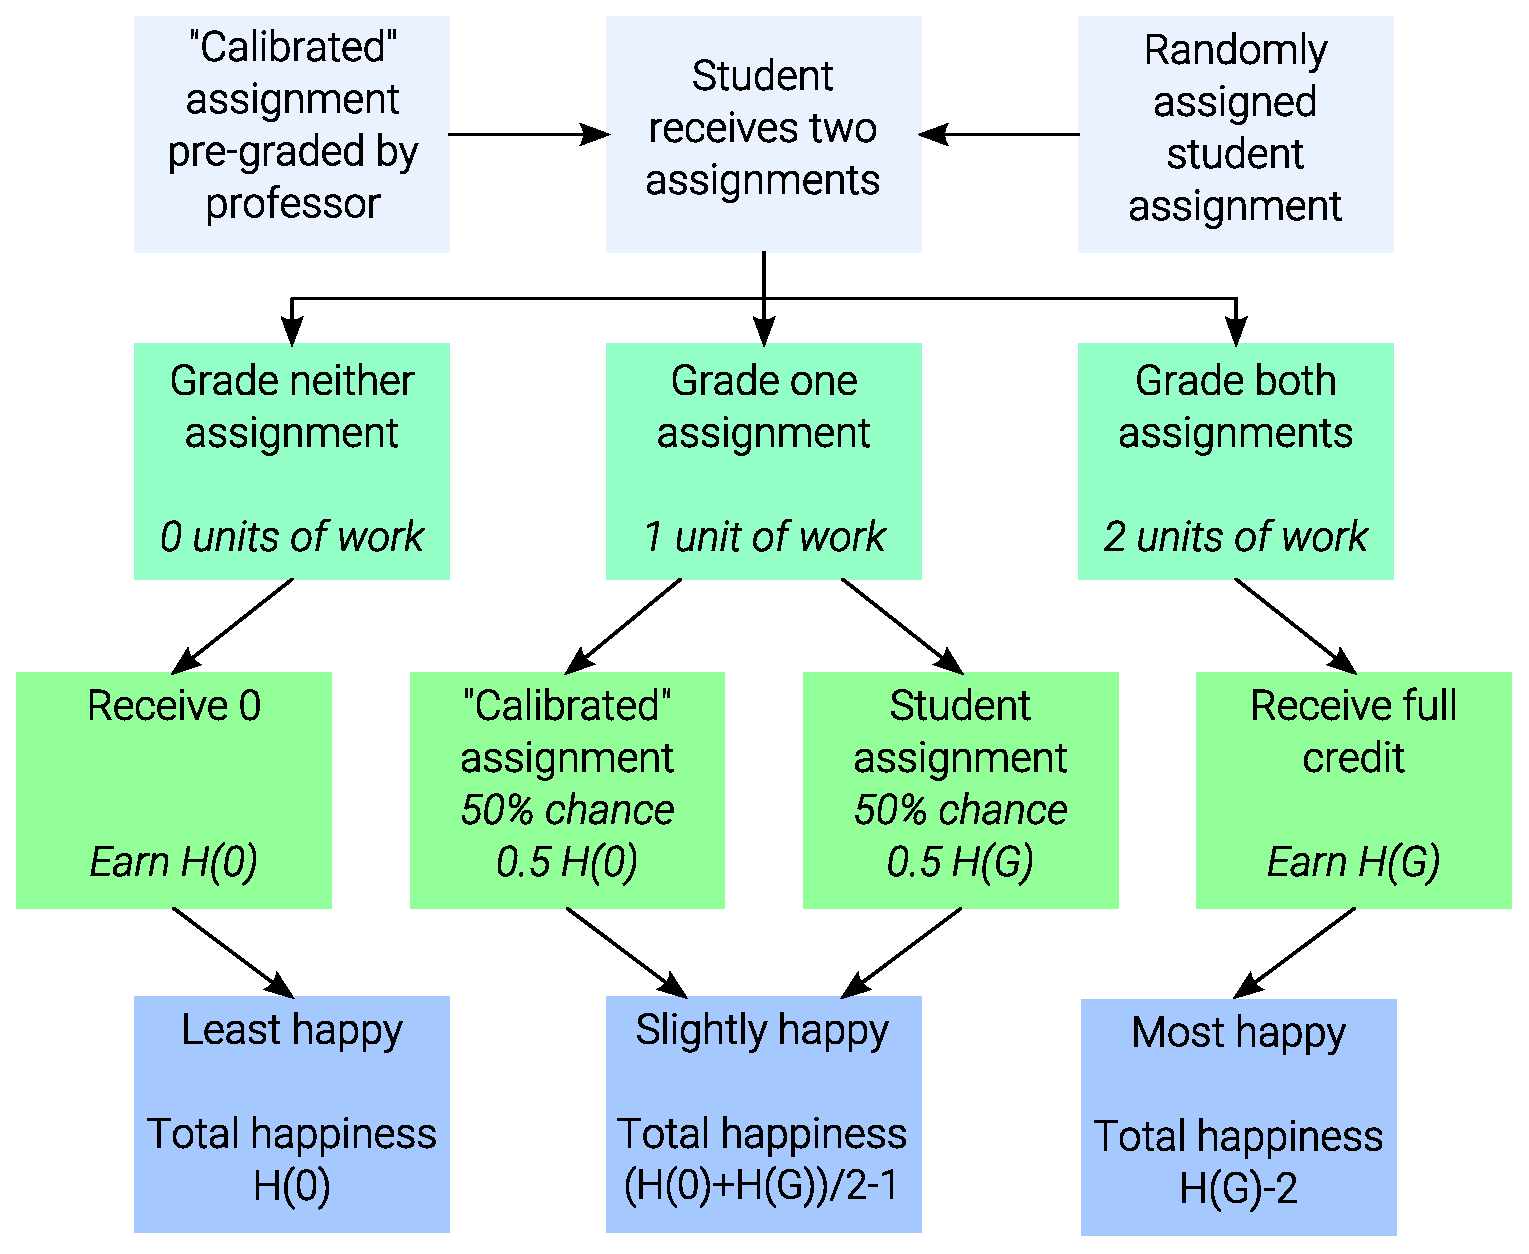
\includegraphics[width=0.9\columnwidth]{Calibration-Flowchart.eps}
\caption{A flowchart of the Calibration Mechanism from the student perspective.}
\label{fig:calibration}
\end{figure}

The Calibration mechanism is described visually in Figure~\ref{fig:calibration}. It achieves a low benchmark score of 4, consisting of a 2 in max work done and 2 in max error in grade.

We tested and verified the Calibration mechanism through an anonymous crowdsourced experiment. In this case, ``grading'' involved counting two sets of objects. Initially unknown to the participant, one set is ``calibrated'' and will be used to reward the participant based on the accuracy of the grading. We added a reward system to the Calibration mechanism to incentivize participants to grade correctly. This reward, awarded for accurately grading the Calibrated set, is synonymous to the punishment administered by the professor upon improperly grading the Calibrated set.

The results of this experiment can be seen in Figure~\ref{fig:error-calibration}, where the maximum error made in grading both calibrated and uncalibrated sets is plotted against the error made only on the calibrated set. The grader's performance on the Calibrated set is shown to be a general indication of the grader's performance overall. Another correlation is evident in Figure~\ref{fig:reward-error}, where grading error is plotted against relative magnitude of reward. This shows that a higher reward correlates to lower error. Together, these verify that the Calibration mechanism indeed works.

\begin{figure}[!h]
\centering
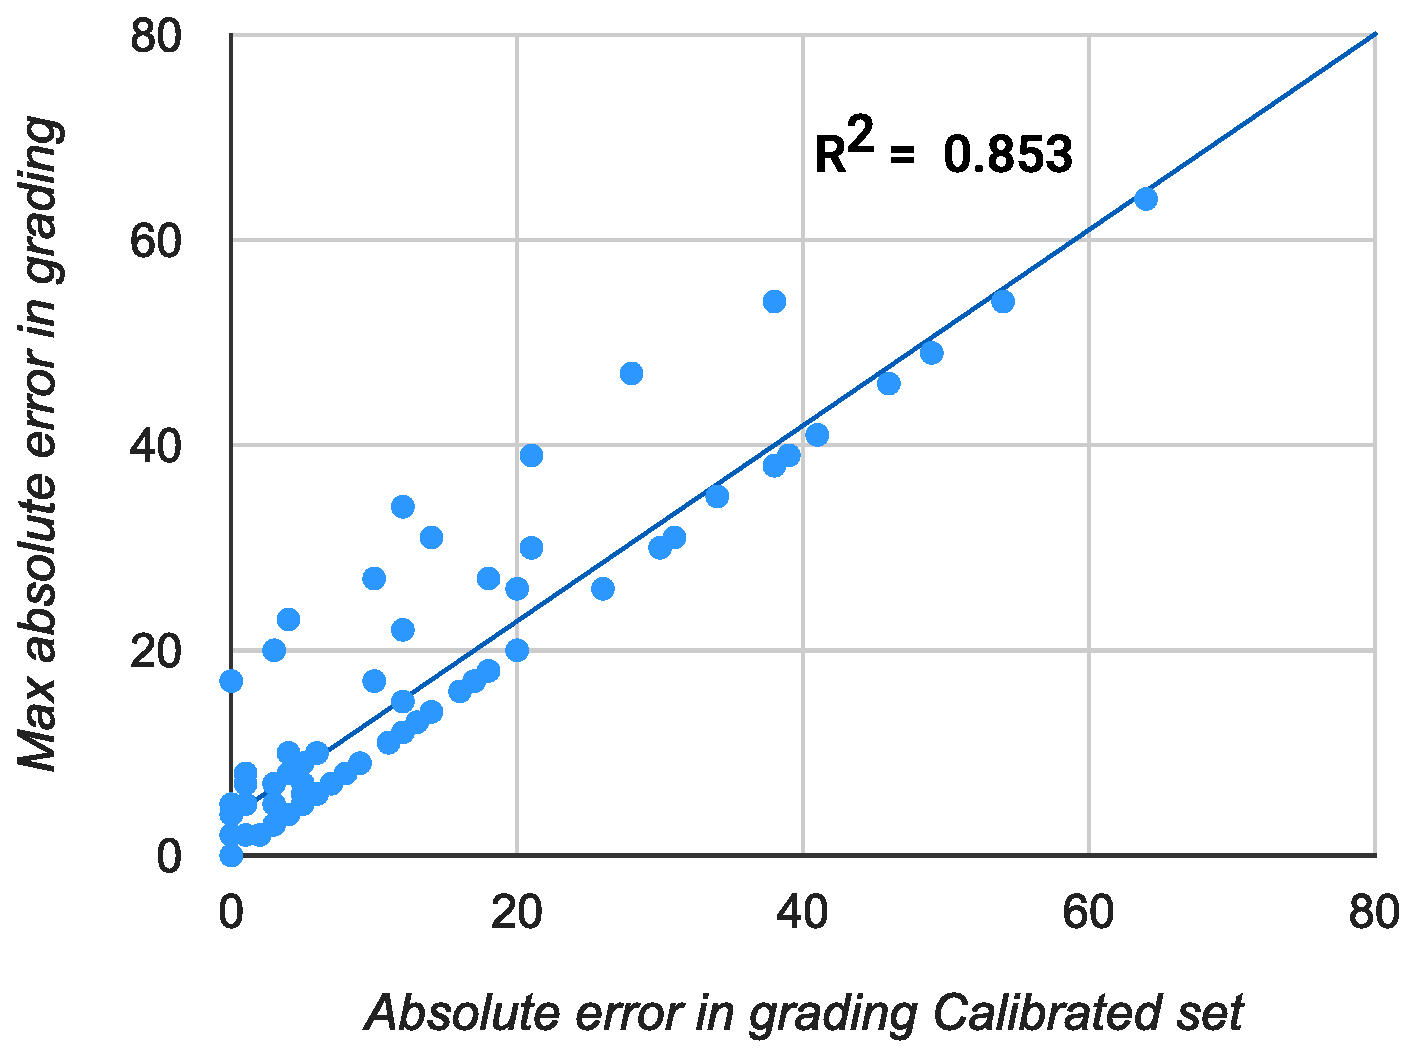
\includegraphics[width=0.9\columnwidth]{Error-Calibration-Graph.eps}
\caption{Max error vs Calibrated error}
\label{fig:error-calibration}
\end{figure}

\begin{figure}[!h]
\centering
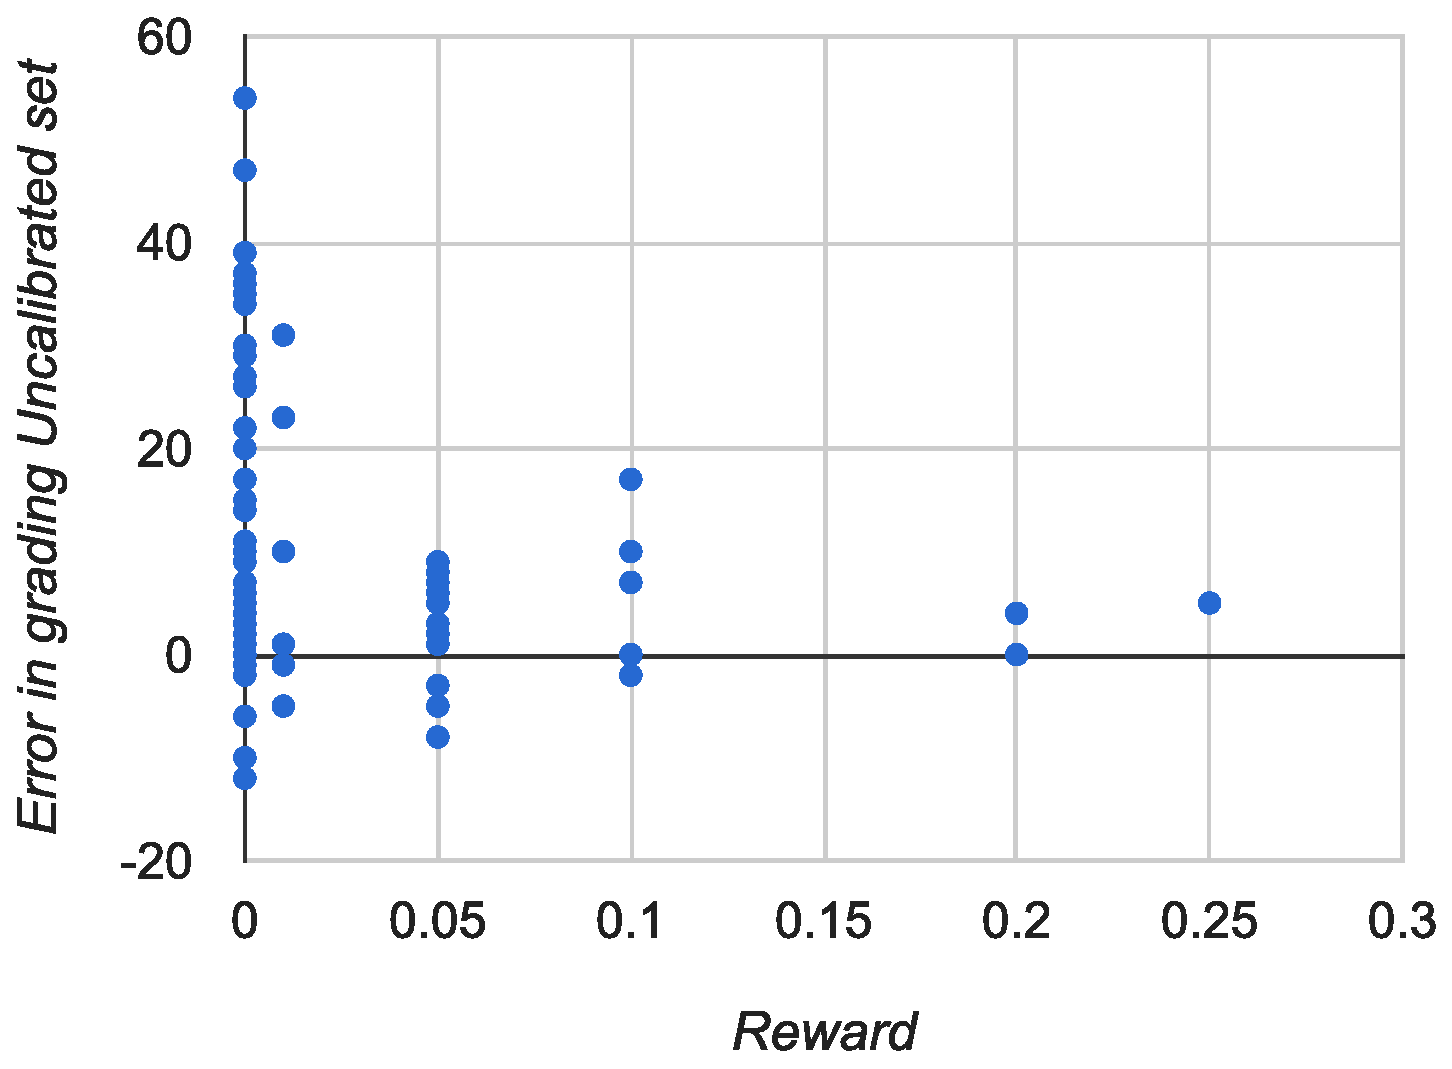
\includegraphics[width=0.9\columnwidth]{Reward-Error-Graph.eps}
\caption{Uncalibrated Error vs Reward}
\label{fig:reward-error}
\end{figure}

Putting two parts together, a grader's overall error can be estimated from performance on the Calibrated set. By rewarding graders based low errors on the Calibrated set, more accurate grades for the uncalibrated set are likely to be attained. Accuracy of grades on the uncalibrated set is one of the goals for the Calibration mechanism, and the data suggests that the mechanism works in practice.

\subsection{Improved Calibration Mechanism}
Originally designed with the assumption that students cannot communicate, the Calibration mechanism quickly breaks when student conspire to reveal the calibrated assignment to circumvent grading. The Improved Calibration mechanism mitigates this issue by introducing multiple calibrated papers at the expense of more work, raising the objective score. However, since the work created by this mechanism does not scale well with class size, a better mechanism was developed: the Deduction mechanism.

\subsection{Deduction Mechanism}

The Deduction mechanism (Figure~\ref{fig:deduction}) achieves a very low benchmark score of 2, with 2 in max work done and a 0 in max error in grade. Incapable graders will raise the benchmark score, as they issue refutations that add work to the professor.

\begin{figure}[!h]
\centering
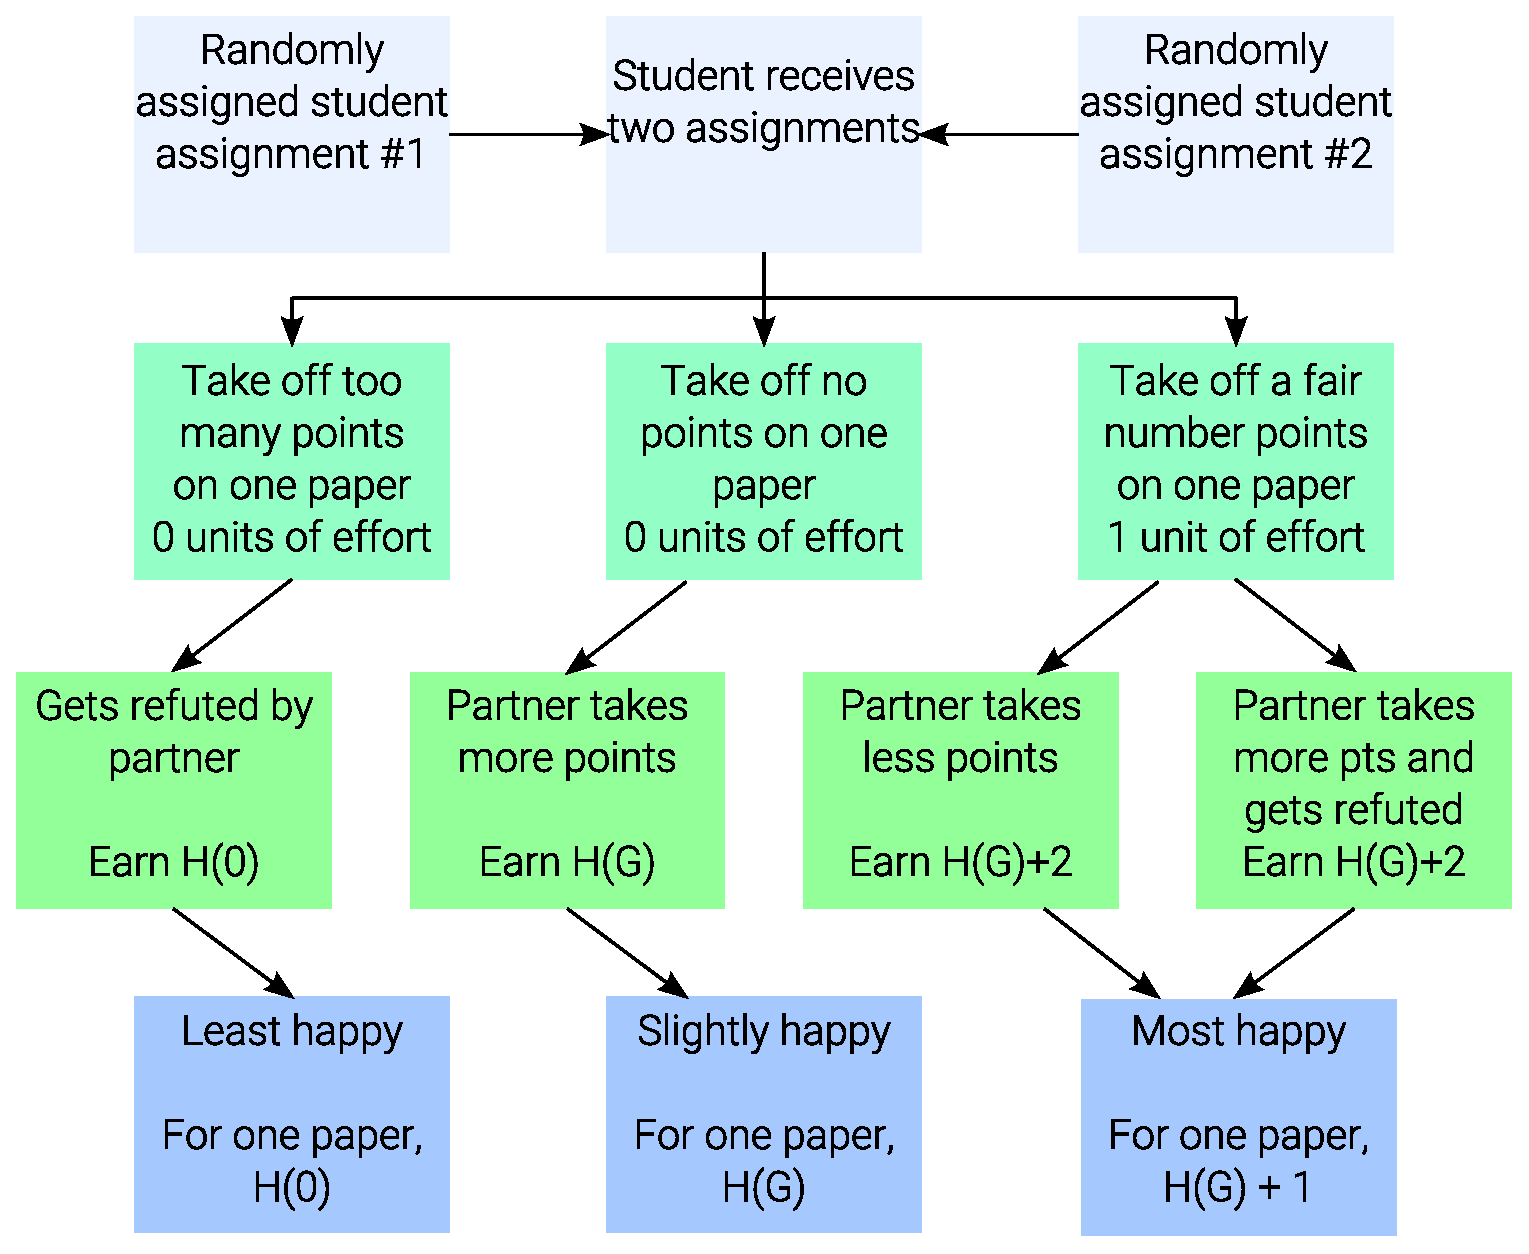
\includegraphics[width=0.9\columnwidth]{Deduction-Flowchart.eps}
\caption{A flowchart of the Deduction Mechanism from the student perspective.}
\label{fig:deduction}
\end{figure}

\section{Results}
The comparison of existing solutions and those proposed in this work can be seen in Figure~\ref{fig:comparison}. Each mechanism will be explained below.

Traditional Professor Grading involves one professor grading all assignments. In an online class of 1000 students, this method is extremely inefficient.

In Traditional Peer Grading, each student grades another's assignment without any supervision. However, as in this mechanism, the objective score is high due to the potential error caused by lack of motivation to grade properly.

% TODO: Add references to computer grading
Although without requiring effort from either professor or student, Traditional Automated Grading of open-ended responses are still under heavy research. Current solutions are quite preliminary, though can arrive at a grade within approximately 25 percent~\cite{automatedsystemssuck}.

The Calibration Mechanism requires one calibrated paper from the professor and two papers graded by each student. The objective score is raised to 4 instead of 2 because students are incentivized by increasing their grade, thus sacrificing accuracy.

The Improved Calibration Mechanism requires each student to grade a subset of the other student's assignments, and the teacher to grade another subset. This mechanism addresses the flaw in the Calibration Mechanism that occurs when students can communicate, at the expense of more work. Thus, leading to poor scalability.

The Deduction Mechanism rewards graders for grading more harshly than their peers, and relies on a voting system to reject grades that are below the expected grade to be reviewed by the professor. In the dominant strategy behavior of the system, no grades should be rejected, leading to no work for the professor. Again, incentive given to the students comes at the cost of accuracy, raising the objective score by two points.

Overall, our Calibration and Deduction mechanisms vastly outperform existing solutions with the exception of Improved Calibration.

\begin{figure}[!h]
\centering
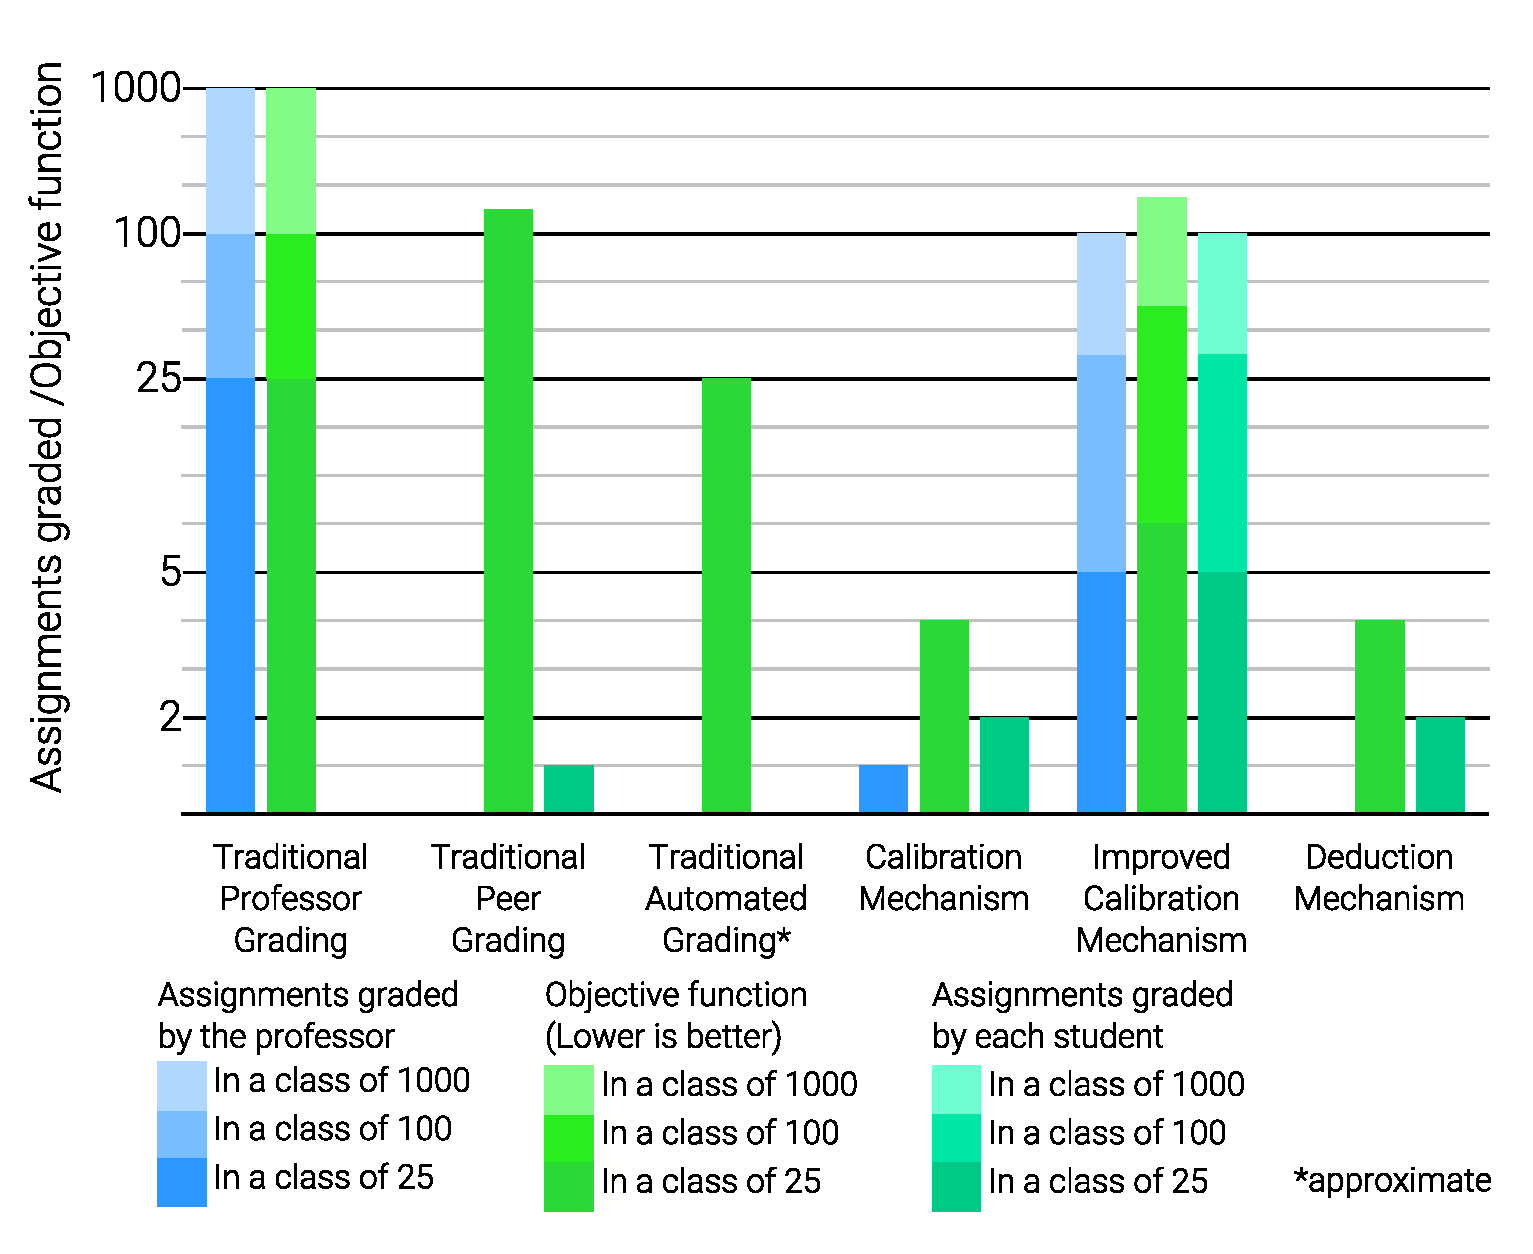
\includegraphics[width=0.9\columnwidth]{Comparison-Graph.eps}
\caption{A comparison of mechanisms in terms of effectiveness and scalability.}
\label{fig:comparison}
\end{figure}



% TODO: Accessibility

% TODO: Prep for Blind Review by removing authors

\section{Conclusion}
An efficient and accurate solution is needed to grade the large number of assignments in MOOCs.

We began by creating a student model - a set of assumptions that approximate the realistic behavior of students. We then developed various grading mechanisms based on our student model and mechanism design. These mechanisms would incentivize students to grade accurately and efficiently as proven by game theory.

We tested our Calibration mechanism using a croudsourced experiment, finding that it could work in practice. A mechanism based on a more realistic model would achieve better results.

Our model can easily be reused and improved upon by future researchers who wish to develop more efficient solutions. Efficiency is measured in terms of the benchmark we created, a numerical score encompassing both the accuracy of grades and the effort spent by any one person. To the best of our knowledge, this is the first game-theory-based peer-grading system.

\section{Future Work}
As we consider how to generate accurate grades from incompetent graders, our model will require more realistic assumptions, which in turn may create more complex mechanisms.
Eventually, we would like to see new mechanisms based off of our model or our existing mechanisms implemented in MOOCs such as EdX or Coursera.


\section{Acknowledgments}
We would like to thank MIT and the MIT PRIMES program for providing the research opportunity as well as our parents and mentors for their support. Of course, none of this is possible without the original idea proposed by our advisor.

\subsection{Additional Authors}
Mentors \newline
\textbf{Matthew~Weinberg}~(\href{mailto:smweinberg@csail.mit.edu}{smweinberg@csail.mit.edu})\newline
\textbf{Christos~Tzamos}~(\href{mailto:ctzamos@gmail.com}{ctzamos@gmail.com})

Advisor \newline
Professor \textbf{Costis~Daskalakis}~(\href{mailto:costis@csail.mit.edu}{costis@csail.mit.edu})


% Note that in a perfect world balance wants to be in the first
% column of the last page.
%
% If balance doesn't work for you, you can remove that and
% hard-code a column break into the bbl file right before you
% submit:
%
% http://stackoverflow.com/questions/2149854/how-to-manually-equalize-columns-
% in-an-ieee-paper-if-using-bibtex
%
% Or, just remove \balance and give up on balancing the last page.
%
\balance

\bibliographystyle{acm-sigchi}
\bibliography{bibliography}
\end{document}
